%\documentclass[tikz, convert]{standalone}
\documentclass[
  tikz, convert={density=800, size=2400x800, outext=.png}, 
  background, border=0.5cm
 ]{standalone}
 \usepackage{amsmath, amssymb, amsthm, xcolor}
\usetikzlibrary{shapes.geometric, positioning}
\usetikzlibrary{quotes, angles, calc, backgrounds}

\tikzset{decisionNode/.style={inner sep=7pt, shape=circle,align=center,font=\Huge,draw, fill=gray!40}}
\tikzset{leafNode/.style={inner sep=7pt, shape=circle, align=center, font = \Huge, draw, fill=white}}
\tikzset{decisionRule/.style={shape=rectangle, align=center, font = \normalsize, draw=none, fill=white}}
\tikzset{jump/.style={shape=rectangle, align=center, font=\Large, draw=none, fill=white}}
\tikzset{annotation/.style={shape=rectangle, align=center, font=\Large, draw=none, fill=white}}

\definecolor{myColor1}{RGB}{153,153,153}
\definecolor{myColor2}{RGB}{230,159,0}
\definecolor{myColor3}{RGB}{86,180,233}
\definecolor{myColor4}{RGB}{0,158,115}
\definecolor{myColor5}{RGB}{240,228,66}
\definecolor{myColor6}{RGB}{0,114,178}
\definecolor{myColor7}{RGB}{213,94,0}
\definecolor{myColor8}{RGB}{204,121,167}

%%
% label placement:
% https://tex.stackexchange.com/questions/333282/how-to-put-text-above-a-node-point-in-tikz

% level spacings to avoid overlaps
% https://tex.stackexchange.com/questions/86919/tikz-tree-without-overlaps


\begin{document}



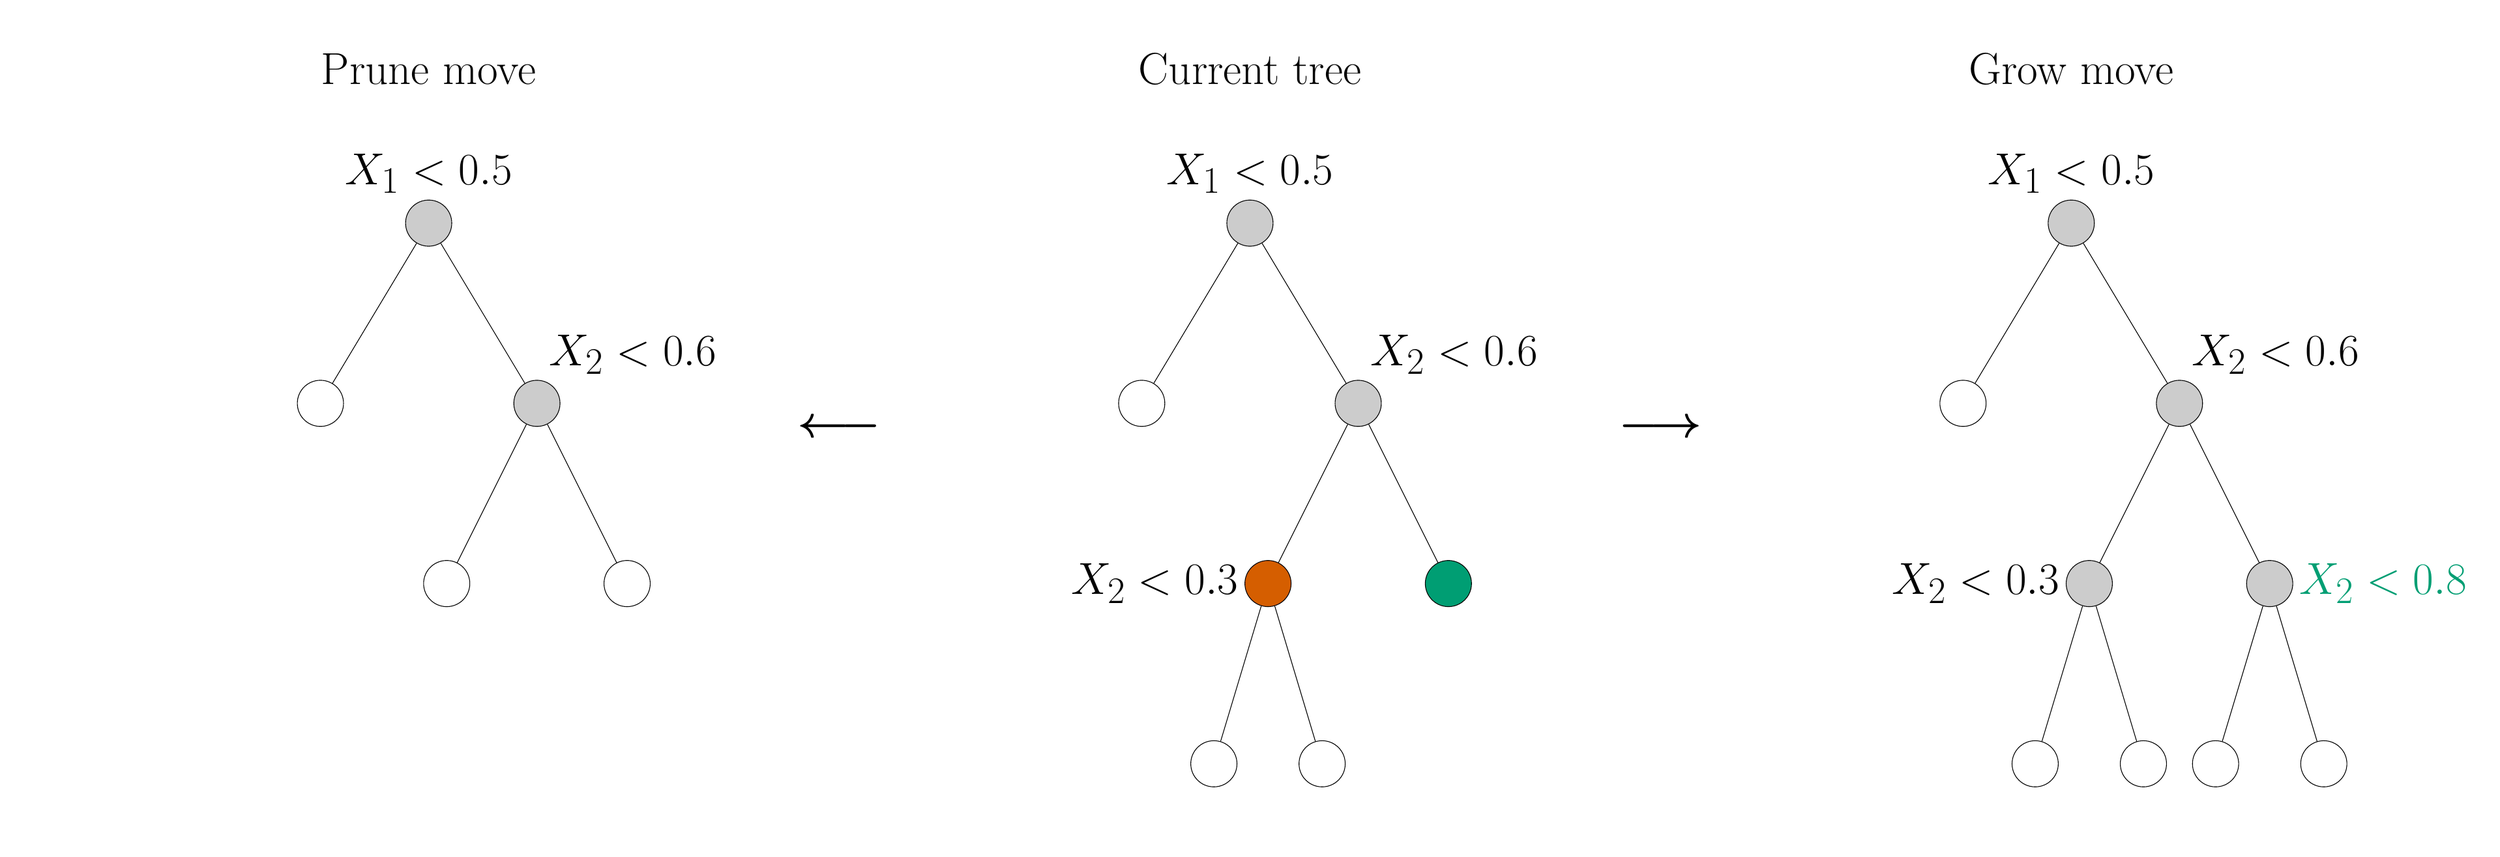
\begin{tikzpicture}[
  background rectangle/.style={fill=white}, show background rectangle,
  level 1/.style={sibling distance = 12em},
  level 2/.style={sibling distance = 10em},
  level 3/.style={sibling distance = 6em},
  level 4/.style={sibling distance = 5em},
  level distance = 10em]
  %sibling distance = 4em, level distance = 4em]
  %sibling distance=4em, level distance = 4em]

\useasboundingbox (-24,-8) rectangle (24,8);
%\draw (0,0) -- (1,0) -- (1,1) -- (0,1) -- (0,0);

% Prune tree
\node[decisionNode, label=above:{\Huge $X_{1} < 0.5$}] (01) at (-16, 4) {~}
  child{ node[leafNode] (02) {~}}
  child{
    node[decisionNode, label=75:{\Huge$X_{2} < 0.6$}] (03) {~}
      child{node[leafNode] (06) {~} }
      child{ node[leafNode] (07) {~} }
  }
;


% Current tree
\node[decisionNode, label=above:{\Huge $X_{1} < 0.5$}] (11) at (0, 4) {~}
  child{ node[leafNode] (12) {~}}
  child{
    node[decisionNode, label=75:{\Huge $X_{2} < 0.6$}] (13) {~}
      child{
        node[decisionNode,fill=myColor7, label=left:{\Huge $X_{2} < 0.3$}] (16) {~}
          child{
            node[leafNode] (112) {~}
          }
          child{
            node[leafNode] (113) {~}
          }
      }
      child{ node[leafNode, fill=myColor4] (17) {~} }
  }
;

% Grow tree
\node[decisionNode, label=above:{\Huge $X_{1} < 0.5$}] (21) at (16, 4) {~}
  child{ node[leafNode] (12) {~}}
  child{
    node[decisionNode, label=75:{\Huge$X_{2} < 0.6$}] (23) {~}
      child{
        node[decisionNode,label=left:{\Huge $X_{2} < 0.3$}] (26) {~}
          child{
            node[leafNode] (212) {~}
          }
          child{
            node[leafNode] (213) {~}
          }
      }
      child{ 
        node[decisionNode, label=right:{\Huge $\textcolor{myColor4}{X_{2} < 0.8}$}] (27) {~}
          child{ node[leafNode] (214) {~}}
          child{ node[leafNode] (215) {~}}
      }
  }
;

\node[annotation] at (-8,0) {\Huge $\boldsymbol{\longleftarrow}$};
\node[annotation] at (8,0) {\Huge $\boldsymbol{\longrightarrow}$};

\node[annotation] at (-16,7) {\Huge Prune move};
\node[annotation] at (0,7) {\Huge Current tree};
\node[annotation] at (16,7) {\Huge Grow move};


\end{tikzpicture}

\end{document}